\section{Implementation Details}
\label{sec:Solution}
In this section, we describe the system architecture and design choices we made. 

\begin{center}
 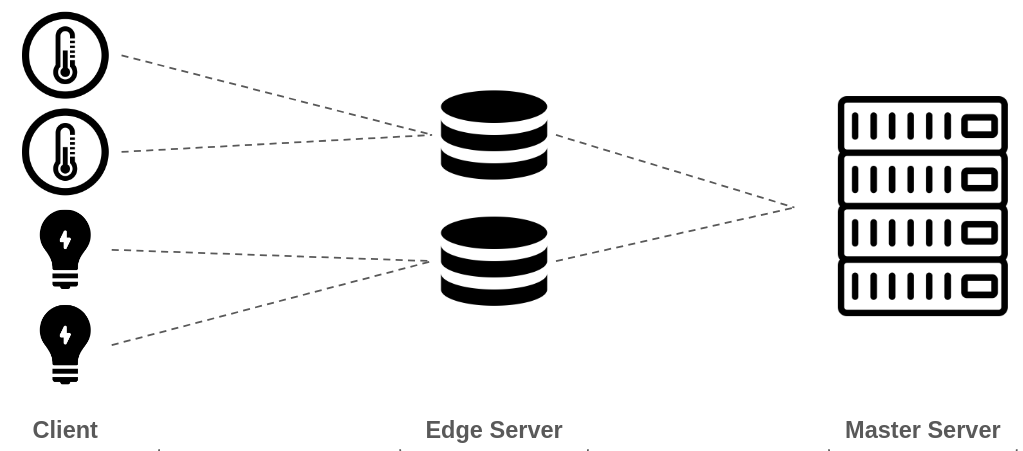
\includegraphics[width=10cm, height=5cm]{sections/Figures/architecture.png}
\end{center}

We implement the whole project in C++~\cite{prj_git}. However, we implement the client service in Python and C++ to compare the two implementations. In the following section, we explain the main components of our system. 
\subsection{Client}
The clients send \texttt{read}, \texttt{write}, and \texttt{delete} requests to the edge servers. In order to improve performance, the clients put \texttt{write} and \texttt{delete} requests in an ordered queue. This allows sending the requests in batches and eliminating redundant requests (e.g., on the same key). Our client implementation runs on two worker threads: a network thread and the main thread.

The main thread collects the data from the environment and initiates the requests to communicate with the edge server. The network thread optimizes and dispatches the requests to the edge servers. For this reason, the main thread can continue to collect data and does not have to work for the network communication--where the network latency can be high.

\subsection{Edge Server}
We implement our key-value store database, which is used heavily by the edge servers. We define three main database queries: \texttt{READ}, \texttt{WRITE}, and \texttt{DELETE}. The main functionality of the edge server is to authenticate clients, execute their queries on the database, and return the query result. In our implementation, we use a REST API with three different endpoints for client-server communication.


\subsection{Master Server}
In our distributed database, it is crucial to guarantee data persistence among edge servers. In order to guarantee a reliable database with low data loss (e.g., in case of a server or network failure), we implement a third architectural component: the master server.

The master server receives backup files from the edge servers and stores them in a secure, permanent disk storage. The master server does not store the backup files in a database object but stores them to--and restores them from--\texttt{json} files.
